\documentclass [11pt, twoside]{article}

%\usepackage{times}
\usepackage{graphicx}
\usepackage{ifthen}
\usepackage{xspace}
\usepackage{fancyhdr}
\usepackage{moreverb}
%\usepackage{hyperref}
\usepackage{float} % for the [H] 
\usepackage{amsmath}
\usepackage{pdfpages}

% solution switch
\newboolean{showsolution}
\setboolean{showsolution}{false}


%layout
\topmargin      -5.0mm
\oddsidemargin  6.0mm
\evensidemargin -6.0mm
\textheight 215.5mm
\textwidth      160.0mm
\parindent        1.0em
\headsep          10.3mm
\headheight        12pt
\lineskip    1pt
\normallineskip     1pt

%header
\lhead{Programming Languages \\ 2021}

\rhead{Prof. O. Nierstrasz\\
Mohammadreza Hazhirpasand, Joel Niklaus}
\lfoot{page \thepage}
\rfoot{\today}
\cfoot{}

\renewcommand{\headrulewidth}{0.1pt}
\renewcommand{\footrulewidth}{0.1pt}

\renewcommand{\thesubsection}{\arabic{subsection}}

%enumeration
\newenvironment{myitemize}{%
     \begin{itemize}
     \setlength{\itemsep}{0cm}}
     {\end{itemize}}

\newenvironment{myenumerate}{%
     \begin{enumerate} \setlength{\itemsep}{0cm}}
     {\end{enumerate}}


%solution
\ifthenelse{\boolean{showsolution}}
   {  \newcommand{\solution}[1]{
   	\noindent\underline{\textbf{Answer:}}\\[2mm]
   	 \textsl{#1}
	 \vspace{10pt}
	 \normalsize
	}
  }
  {  \newcommand{\solution}[1]{} }

\newcounter{exnum}
\def\xexercise{\fontsize{12}{10}\fontseries{bx}\selectfont}
\def\xnormal{\fontseries{m}\fontshape{n}\selectfont}


\newcommand{\exercise}[1]{%
     {\addtocounter{exnum}{1}\vskip 0.8cm{\xexercise \noindent Exercise
\arabic{exnum} (#1)} \xnormal} \vskip 0.3cm} 
 \newcommand{\aufgabe}[1]{
     {\addtocounter{exnum}{1}\vskip 0.8cm{\xexercise \noindent Aufgabe
\arabic{exnum} (#1)} \xnormal} \vskip 0.3cm} 

\pagestyle{fancy}


% ===============ABBREVIATIONS==============================
\newcommand{\eg}{\emph{e.g.,}\xspace}
\newcommand{\ie}{\emph{i.e.,}\xspace}
\newcommand{\etc}{\emph{etc.}\xspace}


\begin{document}

% title
\section*{\ifthenelse{\boolean{showsolution}}{Solution }{}\xspace{}Serie 2 - Postscript}

% - - - - - - - - - - - - - - - - - - - - - - - - - - - - - - - - - - - - - -
\subsection*{Exercise 1}
Answer the following questions about Postscript:

\begin{myitemize}

\item Why would you define your own dictionaries? 
\solution{Dictionaries can be reused, and should help to avoid code
duplication. A pretty good example are the arrows on lecture slide 2.34. - You
can define your own local variables, without having to fear the names have
been used elsewhere.}

\item When should you use \texttt{translate} instead of \texttt{moveto}?
\solution{Translate should be used in conjunction with relative coordinates.
For example, if you define a function which should draw an object starting at
the center of the page (and not at the origin), you should use translate in
order to move the origin to the center. Then the object is drawn relative to
the new coordinate system.}

\item When would you use a matrix instead of \texttt{gsave}/\texttt{grestore}?


\item Why is it important to leave the stack in a consistent state?


\item Implement the equivalent of the following piece of code in postscript:
\begin{verbatim}
public int f(int a, int b) {
    int d = x(a, b);
    z(a, b);
    return d;
}

public int x(int a, int b) {
    return a - b;
}

public int z(int a, int b) {
    return a + b;
}
\end{verbatim}



%\solution{\texttt{gsave} saves the current graphical state}
%\item How could you use dictionaries to simulate object-oriented programming?
%(Give a brief explanation, you don't need to provide any implementation of
%your answer) \solution{}

\end{myitemize}

% - - - - - - - - - - - - - - - - - - - - - - - - - - - - - - - - - - - - - - - - - - - - - - - - - - - - - - - - - - - - - - - - - - -
\subsection*{Exercise 2}

Define a procedure in postscript that will draw a chicken given the following arguments on the stack: 

\begin{enumerate}

\item x and y coordinates of the center of the chicken's body.
\item Radius of the body.
\item Radius of the head.
\item Length of the beak
\item Length of the legs
\item Length of the wings
\end{enumerate}

The call to the procedure should look like this
\begin{verbatim}
% x   y body head beak legs wings
350 400   30   30   30   30    30 chicken
\end{verbatim}

The following pages contain example chickens and the procedure called used to generate them. They where generated by the following postscript code:

\begin{verbatim}

/Times-Roman findfont
18 scalefont
setfont

%%Pages: 4 
%%Page: 1 1
100 700 moveto
(350 400   50   40   30   20    10 chicken) show 
% x   y body head beak legs wings
350 400   50   40   30   20    10 chicken
showpage
%%Page: 2 2
100 700 moveto
(350 400   10   20   30   40    50 chicken) show 
% x   y body head beak legs wings
350 400   10   20   30   40    50 chicken
showpage
%%Page: 3 3
100 700 moveto
(350 400   30   30   30   30    30 chicken) show 
% x   y body head beak legs wings
350 400   30   30   30   30    30 chicken
showpage
%%Page: 4 4
100 700 moveto 
(350 400   80   30   50   40    40 chicken) show 
% x   y body head beak legs wings
350 400   80   30   50   40    40 chicken
showpage
\end{verbatim}

Please use the provided template which contains this code, as it will make it easier for you (and us) to check your solution.

Try to define sub-procedures whenever it makes sense. Please note that the position of the wings and legs should be dependent on the size of the  the chicken's body. Same goes for the position of the beak and eyes with respect to the size of the head. 

Feel free to be creative!

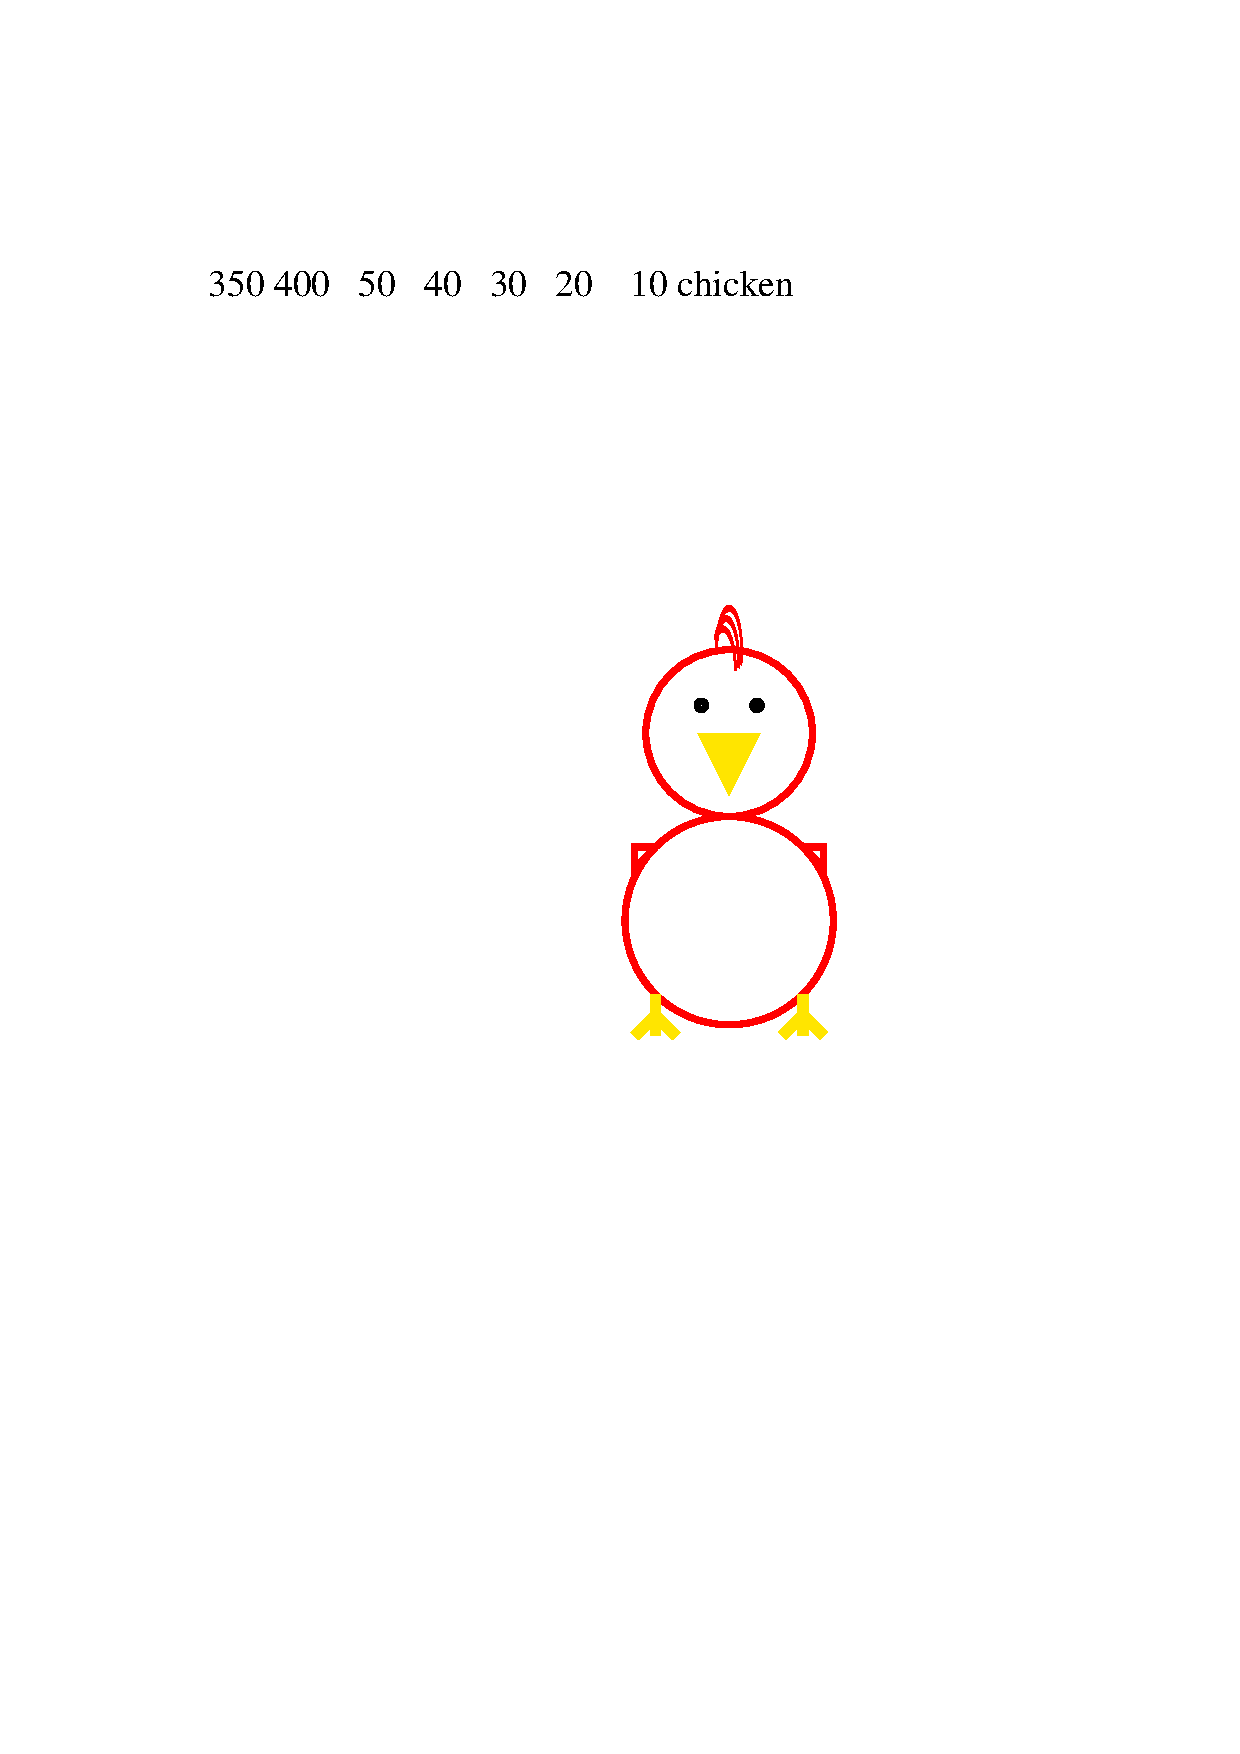
\includepdf[pages=-]{chicken.pdf}


% - - - - - - - - - - - - - - - - - - - - - - - - - - - - - - - - - - - - - - 


\end{document}









